% SOURCE_AUTHORITY: sga5_fr_workpass.tex, lines 1254--1371 (LF-normalized unit).
Veamos ahora que el apareamiento (4.7.1) es \textquotedblleft perfecto\textquotedblright{}, es decir, que la flecha (4.7.1)' identifica $\R\Gamma(V,i_!G')[-1]$ con $\underline{D}_x\R\Gamma(U,G)$. Supongamos, en efecto, como podemos hacerlo, que
\[
G=(ji)^*F,
\]
con $F\in\ob\D_c^b(X)$. Poniendo $F'=\underline{D}_X(F)$ y $F'_{U,X}=(ji)_!G'$, se tiene la sucesión exacta
\[
(4.7.9)\qquad 0\longrightarrow F'_{U,X}\longrightarrow F'\longrightarrow F'|Y\longrightarrow0,
\]
que da lugar a un triángulo distinguido
\[
(b)\qquad
\begin{tikzcd}
& \R\Gamma_x(F'_{U,X}) \arrow[dr] \\
\R\Gamma_x(F'|Y) \arrow[ur,"{+1}"] && \R\Gamma_x(F') \arrow[ll]
\end{tikzcd}
\]
Por definición de $\R\Gamma_x$, se tiene
\[
\R\Gamma_x(F'_{U,X})=\R\Hom(A_x,F'_{U,X});
\]
por tanto, utilizando (4.7.7) y el hecho de que $(F'_{U,X})_x=\R\Gamma(X,F'_{U,X})=0$, se obtiene un isomorfismo canónico
\[
\R\Hom(A_{V,X},F'_{U,X})[1]\xrightarrow{\sim}\R\Gamma_x(F'_{U,X}).
\]
Pero se tiene
\[
\begin{aligned}
\R\Hom(A_{V,X},F'_{U,X})&=\R\Hom(j_!A_V,j_!i_!G')\\
&\xrightarrow{\sim}\R\Hom(A_V,i_!G')\qquad\text{por dualidad (SGAA~3.1.10)},
\end{aligned}
\]
de donde finalmente se obtiene un isomorfismo canónico
\[
(4.7.10)\qquad \R\Gamma(V,i_!G')[-1]\xrightarrow{\sim}\R\Gamma_x(F'_{U,X}).
\]
Por otra parte, se tiene la sucesión exacta
\[
(4.7.11)\qquad 0\longrightarrow A_{U,X}\longrightarrow A_X\longrightarrow A_Y\longrightarrow0,
\]
que da lugar a un triángulo distinguido
\[
(a)\qquad
\begin{tikzcd}
& \R\Gamma(U,F|U) \arrow[dl,"{+1}"'] \\
\R\Gamma_Y(F) \arrow[rr] && \R\Gamma_X(F) \arrow[ul]
\end{tikzcd}
\]
En virtud de (4.7.1) y (4.7.10), se tiene un apareamiento natural
\[
(4.7.12)\qquad \R\Gamma(U,F|U)\times\R\Gamma_x(F'_{U,X})\longrightarrow A.
\]
En virtud de (4.6.1), se tiene un apareamiento perfecto
\[
(4.7.13)\qquad \R\Gamma_Y(F)\times\R\Gamma_x(F'|Y)\longrightarrow A.
\]
Por último, por la fórmula de inducción ordinaria (1.12 b) (i)), se tiene un apareamiento perfecto
\[
(4.7.14)\qquad \R\Gamma(X,F)\times\R\Gamma_x(F')\longrightarrow A.
\]
El lector que tenga la paciencia de orientarse en este dédalo de \textquotedblleft flechas canónicas\textquotedblright{} comprobará que los apareamientos (4.7.12), (4.7.13) y (4.7.14) son \textquotedblleft compatibles\textquotedblright{} con las flechas de los triángulos (a) y (b), y, por consiguiente, que los apareamientos (4.7.12) y (4.7.1) son perfectos.

El apareamiento de los triángulos (a) y (b) da lugar a dos sucesiones exactas \textquotedblleft transpuestas una de la otra\textquotedblright{}:
\[
(4.7.15)\qquad \cdots\longrightarrow \H_Y^i(X,F)\longrightarrow\H^i(X,F)\longrightarrow\H^i(U,F)\longrightarrow\cdots
\]
\[
\cdots\longleftarrow \H_x^{-i}(Y,F'|Y)\longleftarrow\H_x^{-i}(X,F')\longleftarrow\H^{-i-1}(V,F'_{U,V})\longleftarrow\cdots.
\]
En resumen, podemos enunciar:

\begin{statement}{Proposición 4.7.16}
Sea $X$ un esquema estrictamente local noetheriano, de punto cerrado $x$. Sean $Y$ un cerrado no vacío de $X$, $U=X-Y$, $V=X-x$, e $i:U\to V$ y $j:V\to X$ las inclusiones canónicas. Sea $K_X$ un complejo dualizante sobre $X$ normalizado en $x$ (de donde se obtienen complejos dualizantes asociados sobre $V,U,Y$). Para $G\in\ob\D_c^b(U)$, se tiene un apareamiento perfecto:
\[
(*)\qquad \R\Gamma(U,G)\times\R\Gamma(V,i_!G')[-1]\longrightarrow A
\]
(donde $G'=\underline{D}_U(G)$). Si $G=F|U$, donde $F\in\ob\D_c^b(X)$, se tiene un isomorfismo canónico
\[
(**)\qquad \R\Gamma(V,i_!G')[-1]\xrightarrow{\sim}\R\Gamma_x(F'_{U,X})
\]
(donde $F'=\underline{D}_X(F)$ y $F'_{U,X}=(ji)_!(F'|U)=(ji)_!(G')$), y un apareamiento perfecto entre los triángulos distinguidos
\begin{center}
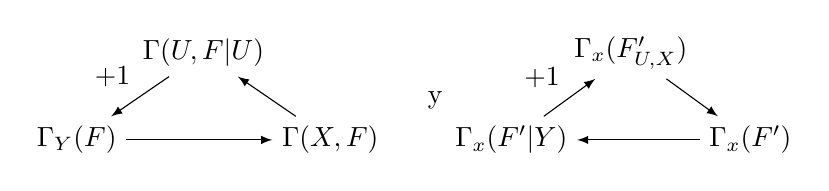
\begin{tikzpicture}[>=latex,scale=0.92,baseline=(current bounding box.center)]
\node (aT) at (0,1.2) {$\R\Gamma(U,F|U)$};
\node (aL) at (-1.75,0) {$\R\Gamma_Y(F)$};
\node (aR) at (1.75,0) {$\R\Gamma(X,F)$};
\draw[->] (aL) -- (aR);
\draw[->] (aR) -- (aT);
\draw[->] (aT) -- node[above left] {$+1$} (aL);
\node at (3.2,0.55) {y};
\node (bT) at (5.9,1.2) {$\R\Gamma_x(F'_{U,X})$};
\node (bL) at (4.25,0) {$\R\Gamma_x(F'|Y)$};
\node (bR) at (7.55,0) {$\R\Gamma_x(F')$};
\draw[->] (bT) -- (bR);
\draw[->] (bR) -- (bL);
\draw[->] (bL) -- node[above left] {$+1$} (bT);
\end{tikzpicture}
\end{center}
compatible con el apareamiento $(*)$ y el isomorfismo $(**)$, y que da lugar a dos sucesiones exactas transpuestas una de la otra (4.7.15).
\end{statement}

\begin{statement}{Observación 4.7.17}
En el caso particular en que $Y=\{x\}$, el apareamiento (4.7.1) se define bajo la sola hipótesis de que $K_X$ esté normalizado en $x$ (y no necesariamente sea dualizante), es decir, que $\R\Gamma_x(K_X)\simeq A$ (dándose el isomorfismo): en efecto, el isomorfismo (4.7.2) (que utilizaba la bidualidad) se reduce a la identidad. Como el apareamiento (4.7.14) es perfecto en cualquier caso, se ve, pues, que la dualidad local sobre $X$ (en la forma (4.2.2)') equivale a la dualidad \textquotedblleft global\textquotedblright{} sobre $U=X-x$, es decir, al hecho de que el apareamiento (4.7.1)
\[
\R\Gamma(U,G)\times\R\Gamma(U,G')[-1]\longrightarrow A
\]
sea perfecto, o, equivalentemente, que los apareamientos
\[
\H^i(U,G)\times\H^{-i-1}(U,G')\longrightarrow A
\]
sean perfectos.

Supongamos que se dispone sobre $X$ de un complejo dualizante $K_X$ normalizado en $x$. Si $X$ es excelente y $U$ regular de dimensión $d$ (de modo que $x$ puede ser una singularidad aislada), debe poder verificarse que $K_U=K_X|U$ es canónicamente isomorfo a $(\mu_n)_U^{\otimes d}[2d]$ (se verifica fácilmente, en todo caso, si $X$ es la localización estricta de un esquema localmente de tipo finito sobre un cuerpo de car.~0). Entonces la dualidad local sobre $X$ implica que, para todo $A_U$-módulo localmente constante constructible $G$, se tienen apareamientos perfectos:
\[
\H^i(U,G)\times\H^{2d-1-i}(U,G^\circ)\longrightarrow A,
\]
(donde $G^\circ=\uHom(G,(\mu_n)_U^{\otimes d})$), que corresponden formalmente a la dualidad de Poincaré sobre un esquema de dimensión $2d-1$.
\end{statement}
